\documentclass[12pt, a4paper]{article}
\usepackage[margin=1in]{geometry}
\usepackage[utf8]{inputenc}
\usepackage[default,scale=0.95]{opensans}
\usepackage{biblatex}
\usepackage{titlesec}
\usepackage{graphicx}
\usepackage{parskip}
\usepackage{xcolor}
\usepackage{hyperref}

\hypersetup{%
  colorlinks=true,% hyperlinks will be coloured
  linkcolor=black,% hyperlink text will be black
  linkbordercolor=red,% hyperlink border will be red
}

\newenvironment{question}
    {\begin{center}
    \begin{tabular}{p{0.9\textwidth}}
    }
    {
    \end{tabular} 
    \end{center}
    }

\newcommand{\technology}[1]{\textit{\textbf{#1}}}
\newcommand{\ipvsix}{IPv6}
\newcommand{\lora}{LoRa}
\newcommand{\bluetooth}{Bluetooth}
\newcommand{\ble}{\bluetooth{} Low Energy}
\newcommand{\wifi}{WiFi}
\newcommand{\bles}{BLE}
\newcommand{\iot}{IoT}
\newcommand{\http}{HTTP}
\newcommand{\coap}{CoAP}
\newcommand{\gap}{GAP}
\newcommand{\gatt}{GATT}
\newcommand{\uri}{URI}

\addbibresource{references.bib}

\setlength{\parindent}{0pt}
\title{Internet of Things - BLE V5.0}
\author{Mathieu Coussens \and Pieter De Clercq \and Freija Verbeke}
\date{\today}

\begin{document}

\pagenumbering{gobble} 

\maketitle
\newpage
\tableofcontents

\newpage
\pagenumbering{arabic}
\setcounter{page}{1}

\section{Introduction}
In this report, we will investigate how \ble{} \emph{(\bles)} can be applied in medical grade monitoring equipment. We propose a prototype and minimal working example that connects a wearable to a cloud platform, through the use of another device with \bles{}- and Internet capabilities, such as a smartphone or a computer. This prototype will be outlined in \autoref{sec:prototype}.

Before going into detail about the specifics of the prototype, we will first take a look at the specifications of \bles{} and consider two alternative protocols: \lora{} and \wifi{}. For \bles{}, the impact on smartphones and computers will also briefly be discussed. In order to provide the reader some more intuition for possible usages, we will also consider some different kinds of wearables and how these can be facilitated by \bles{}.

In \autoref{sec:eval} we will briefly evaluate the performance of the prototype and address some of the questions that may arise when working with \bles{}. At last, \autoref{sec:concl} will contain our main conclusions and the lessons we have learned while working on this project.

\subsection{Network technologies}
\subsubsection{\ble{}}
\bles{} is a new version of Bluetooth, specifically designed with \iot{}-devices like our wearables in mind. Instead of having a power consumption of 1 W like traditional \bluetooth{}, \bles{} only consumes 0.01-0.5 W, cutting battery usage in half. Bluetooth can achieve data rates of up to 24 Mbit/s, however \bles{} can only achieve a data rate of 2 Mbit/s, with a maximum transmission power of 100 mW. The amount of slaves that can connect to a single \bles{} master node is implementation dependent, which allows for a higher level of flexibility. Compared to the range of 10m supported by its predecessors, \bles{} supports ranges up to 100m. Since we will investigate wearables, this is more than sufficient for our use case. Having a larger range would also cause a diminishing effect on the achievable data rate because of interference from other devices.

Technically, \ble{} consists of two important concepts: Generic Access Profile (\emph{\gap}) and Generic Attribute Profile \emph{\gatt}\cite{townsend_2014}. \gap{} defines the role of the device. Various roles exist, but essentially a device can be classified either as a \emph{Central} device, a \emph{Peripheral} device, or even both simultaneously. Peripheral devices, also referred to as ``slaves'', are small, low power \iot{} devices, such as wearables. They typically consist of one or more sensors and report their values to an associated central device. This central device is usually a more powerful device with additional connectivity besides \bles{}, in our prototype this will be a computer. \gatt{} refers to the semantics of how data is formatted and structured. It is possible to create a scheme by yourself, but the protocol also has various schemes already built-in, examples include blood-pressure measurements, heart-rate measurements, and velocity.

The biggest downside of using \bles{} is the fact that direct communication with the internet is not possible from a peripheral node. There is a need for a central node with internet connectivity, in the form of a smartphone or computer in our case. Furthermore, since \bles{} 5 has only been released in 2017, there is a high chance that your smartphone or laptop will not yet support it.

\begin{figure}[htbp]
	
\includegraphics[width=0.5\textwidth]{images/bluetooth.pdf}
	\centering
	\caption{\bluetooth{} logo}
\end{figure}

\subsubsection{\lora{}}
Long Range Wide Area Network, abbreviated as \lora, is a network technology that enables long-range transmissions with low power consumption. It has a rather small bandwidth and has a data rate between 0.3 and 27 kbit/s \cite{lorapaper}. This can provide useful if a permanent connection is not necessary (e.g. a hourly measurement) and if the amount of transmitted data is not too much, since \lora{} only allows 10 messages to be retrieved per day. Besides this, it allows a data range of several kilometers. \lora{} has good coverage in over 100 countries, specifically for Belgium the entire country is covered by Proximus. Unlike \ble{}, direct connection with a cloud platform is possible.

\begin{figure}[htbp]
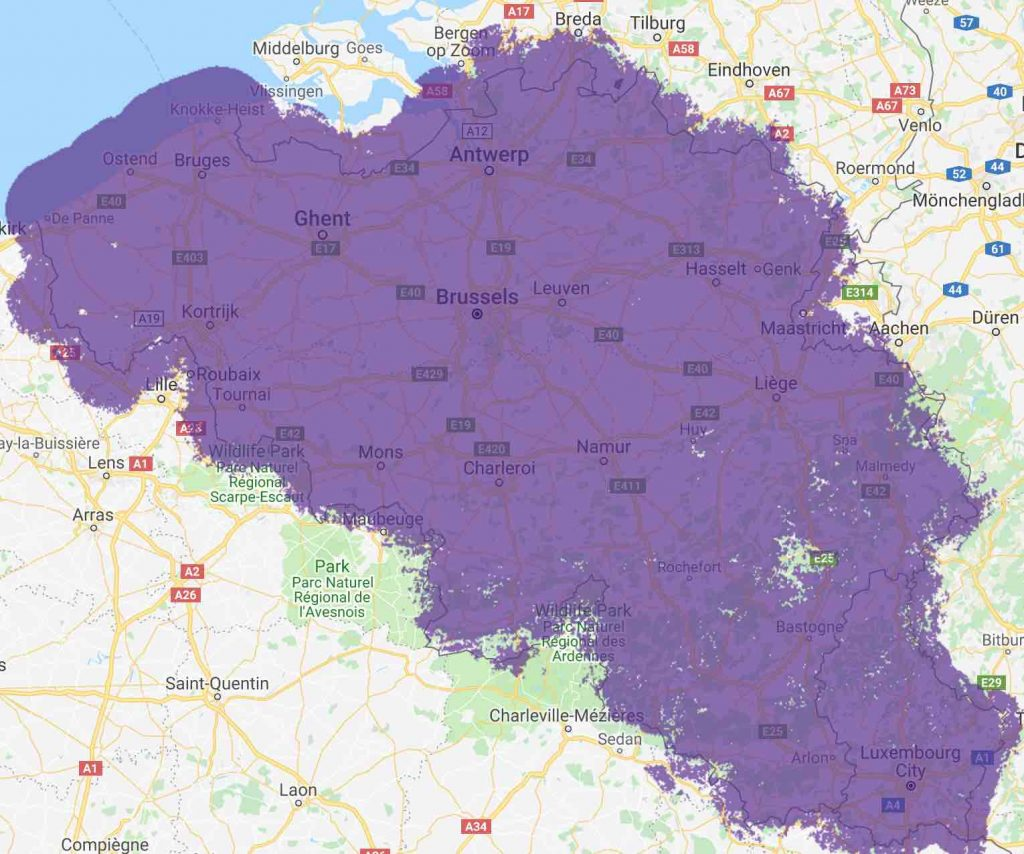
\includegraphics[width=0.75\textwidth]{images/proximus-lora-coverage.jpg}
\centering
\caption{\lora{} coverage in Belgium by Proximus}
\end{figure}

\subsubsection{\wifi{}}
\wifi{} is a family of wireless networking technologies, based on the IEEE 802.11 family of standards, which are commonly used for local area networking of devices and Internet access. \wifi{} can achieve very high data rates of several hundreds of Mbit/s, depending on the distance to the access point.

These high data rates, along with the ability to connect directly to the internet, are the main advantages of using \wifi{}. However, this comes at a cost. \wifi{} demands a high power consumption, nullifying its applicability in \iot{}, since one of the goals is to make the battery last as long as possible. Another disadvantage is the coverage. One might argue that the coverage of \wifi{} is excellent. This is partially true, since nowadays almost every household has a \wifi{}-network and all major cities also have public \wifi{}-networks available. However, there also exist areas without any \wifi{}-networks and these public \wifi{}-networks that do exist, often pose slow data rates, block various connection types, or have questionable reliability. From an end-user point of view, this would also imply that every time you want to go outside and connect to a new \wifi{}-network, you have reconfigure your \iot{} device with the new \wifi{} credentials.

\subsubsection{Bluetooth Mesh}
\ble{} now also supports mesh networking. This means that a node attempts to connect to as many other nodes as possible, in order to create a network of nodes that allows to cover a large distance by means of hopping through other nodes. Essentially this extends the range of \bles{}.

\begin{figure}[htbp]
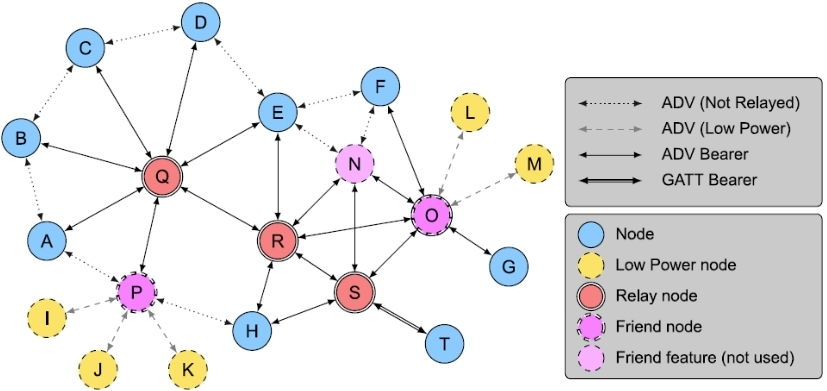
\includegraphics[width=0.9\textwidth]{images/bt_mesh_topology.jpg}
\centering
\caption{\bluetooth{} mesh}
\end{figure}

\newpage

\subsection{Wearables}
\label{wearables}
Before explaining how we will connect the wearables to the cloud platform, we will quickly summarize the different types of wearables we considered when designing our prototype. Other possibilities for these wearables will briefly be mentioned.

The first and most common wearable is a blood pressure and heart rate monitor. These devices are usually worn around the wrist like a watch. Connecting them to the internet can provide some useful services, such as informing your doctor when you have a high blood pressure or even detect anomalies in your heart rate patterns. For this type of wearable, it is important that the data is (near) reported real-time, thus requiring a stable connection. This data can also be visualised as plots, to generate some statistics, such as daily averages, providing the user with a better overview of their physical health. Besides yourself, this can also provide doctors with useful insights, since the results will be more accurate if they are measured over a longer time as opposed to once during a doctors consult.

A second wearable to be considered are sleep monitors. This is an example of data that doesn't have to be real-time. Most \iot{} devices are not capable of storing a lot of data because their RAM (or even ROM) isn't big enough, so storing non-aggregated data for a whole night might not be possible. For this type of wearables, a trade-off needs to be made between storing the data and sending the data. Remark that sleep monitors are often also included in a device with blood pressure and heart rate monitors.

A third type of wearable is a fitness-wearable, that tracks the amount of calories burned, the heart rate under exercise, blood pressure, and other useful values. Because of the large amounts of data, \wifi{} is the best pick if real-time data retrieval is required. Putting this to practice, a fitness centre could be equipped with \wifi{} routers and possibly provide their own cloud platform where customers could track their data.

\section{Prototype}
\label{sec:prototype}

Our architecture consists of 3 main components:
\begin{enumerate}
    \item The peripheral/sensor device
    \item A \bles{}-central border router (laptop)
    \item A cloud platform that collects data sent out by each of the sensors
\end{enumerate}

\begin{figure}[htbp]
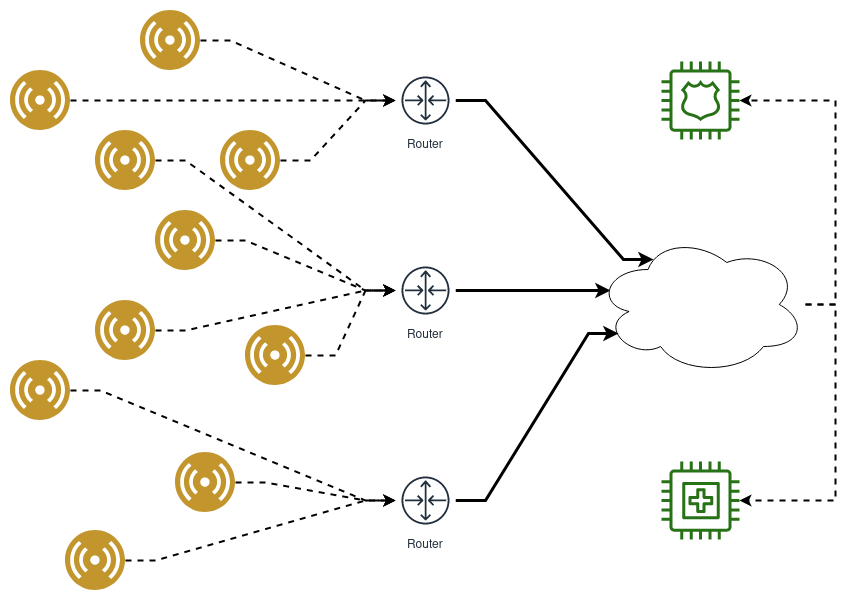
\includegraphics[width=0.8\textwidth]{images/architecture.png}
\centering
\caption{Architecture (including emergency services that read the data on the cloud platform)}
\end{figure}

\subsection{Peripheral (sensor) device}
The \iot{} sensor device performs measurements using sensors, collects those values and sends them over the air via the chosen network technology (\bles{}, \lora{}, Zigbee, \ldots). This device is often light and tiny, its physical form factor would most likely depend on the size of the measuring apparatus inside the device. Examples of data that can be collected by these sensors is insulin and blood sugar levels, heart rate, blood pressure, blood oxygen saturation, \ldots

In our prototype, we have used \bles{} on a Nordic nRF52 device. Since this device does not come with an actual heart rate sensor, we have simulated one using a linear random generator that generates a random value every second, based on the previous generated value and within two configurable bounds. The device communicates its current status using the onboard LEDs. The LEDs blink intermittent when the device is ready to accept a connection, when it is connected the LEDs are off. If it is connected to a border router, it will broadcast a new heart rate value measurement every second using a custom \gatt{} profile, in which every heart rate measurement is encoded in 1 byte.

\subsection{Central device / Border router}

The job of this device is to act as a relay between the peripheral device and the cloud platform. The border router first connects to the wearable and subsequently subscribes to its measurement of interest. Every once in a while, this data is transformed into a standard web format such as JSON\footnote{JavaScript Object Notation}, and eventually transmitted to the cloud platform. If this would be implemented as a mobile application, this could be useful in a hospital setting for heart patients. If every patient can be assigned a wearable heart rate monitor, this could help them become more mobile and less bedridden, as they don't have to lug around a large dedicated heart rate monitor. This could subsequently decrease medical complications, muscle loss or bedsores.

In our setup, this device is implemented as a daemon which is running on a laptop. It has an internal buffer with a configurable buffer size that, when filled, is flushed to the cloud platform. In case real-time information is necessary, the size of this buffer can simply be put to zero, disabling the buffer. Every 5 seconds (regardless of the buffer size), the daemon contacts the cloud platform to fetch the parameter values (see \autoref{ssec:cloud-platform}). If these have changed, the updated values are pushed to the peripheral.

\subsection{Cloud platform}
\label{ssec:cloud-platform}

We have implemented the cloud platform as a simple Node.js application that listens over HTTP for POST requests originating from the border router. The platform also allows the user to configure parameters that are then sent to the device using the border router, thus enabling bi-directional communication. For our prototype, since we are using a simulated heart rate generator, the configurable parameters are the lower and upper bounds of the random generated heart rate measurements.

In practice, using actual parameters, this would save the wearer of the peripheral from having to visit the doctor or go through a rather complicated firmware update process, since the doctor could simply change the required parameters using the cloud platform. An example of a parameter value could be the rate at which measurements are sampled. Some patients may pose a higher risk of heart failure and thus require a higher update frequency so that the cloud platform could inform emergency services if required.

\begin{figure}[htbp]
	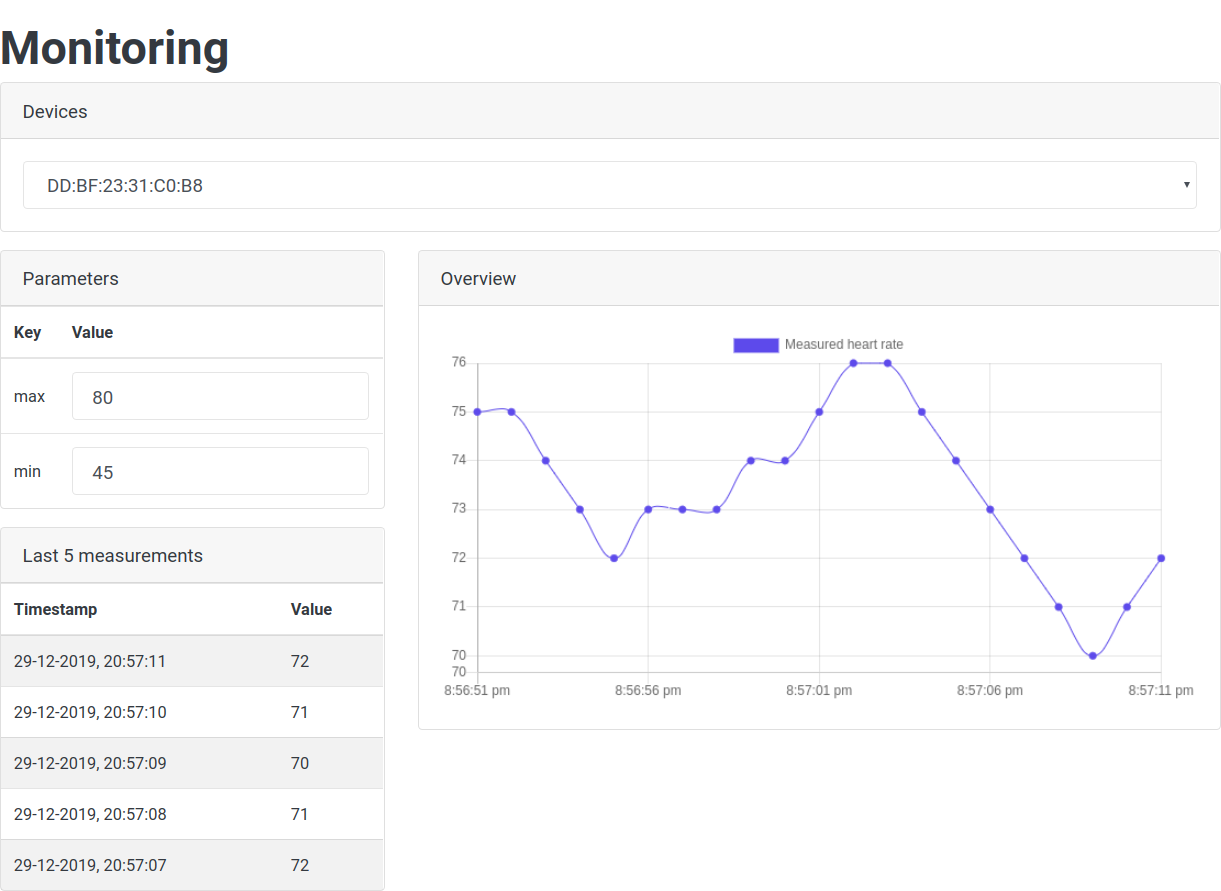
\includegraphics[width=\textwidth]{images/cloud-platform.png}
	\centering
	\caption{User interface of the cloud platform}
\end{figure}

\section{Evaluation}
\label{sec:eval}

\subsection{Q1: Sensor data}

\begin{question}
How much sensor data can be sent to the smartphone (i.e. which data rates can be supported)? Is there an impact on the battery lifetime? Please motivate.
\end{question}

The theoretical limit of the bandwidth is 2Mbit/s, however, since every measured heart rate in our prototype can be encoded as 1 byte, we only require a data rate of 8 bit/s. Since we have assumed a real-time example of a heart rate monitor, the radio cannot be interrupted (as this would also break the connection), so the battery usage remains between 0.05-0.5 W.

\subsection{Q2: Ease of getting data to cloud platform}

\begin{question}
Can we easily get the data to a Cloud platform (e.g. to track the status of the devices). What is the possibility to use end-to-end \ipvsix{} connectivity?
\end{question}

It would be possible to use end-to-end \ipvsix{} connectivity, if one would opt for a protocol such as 6LoRaWAN \cite{8217061}. This does however require the sensor device to be compatible with \lora{} as a transmission technology and \ipvsix{} as the routing protocol. This would cut out the border router as a middle man, as pretty much any web technology would (should) be able to run on top of \ipvsix{}, provided that the sensor device has the computational capacity to transmit the data in a format interpretable by the cloud platform.

\subsubsection{Message Broker}

We also theoretically explored the possibility of increasing the scalability of our cloud platform by putting a message broker in between the sensor and the cloud platform. A good, open source technology that provides this functionality is RabbitMQ\footnote{\url{https://www.rabbitmq.com/}}. The inclusion of a message broker in our pipeline would only be useful for data-sensing that is not dependent on the fact that everything is processed real-time. We would not want the data of a heart attack victim to be held in a message broker for a minute. This would impose severe risks for the health and safety of the patient.

However, an application such as sleep monitoring could potentially benefit from having a simple message broker in between the sensor and cloud platform. The sensor can push data to the message queue and deal with the data quickly. At the end of the night, the cloud platform could then pull the data from the message queue and start the batch processing. A couple of hours later, the data can be made available to the doctor for further analysis.

As such, if the cloud platform takes longer than a specified amount of time to process all data, it could spin up an extra worker to help spread the computational load. This would ensure that all data is processed in a usable time frame, and no component of the system is ever being blocked by a long computation.

\subsection{\coap{}}

As this question assumes that we have end-to-end \ipvsix{} connectivity, we have a choice to make for the application layer protocol. We could go for standard \http{} or use a similar protocol that is designed more for constrained devices: \coap{}. This protocol has a lot of similarities in terms of the actual data that is being sent. It is also based on various methods that perform some action on a \uri{}, which ultimately could change the state of a resource.

Our prototype cloud-platform however has been coded to accept \http{} requests, but could accept \coap{}-requests using middleware\footnote{\url{https://github.com/mcollina/node-coap}}.

\subsection{Q3: Passing equipment from user to user}

\begin{question}
Can the equipment be easily passed from one user to another (e.g. what is the impact on user commissioning, configuration, link with Cloud platform)?
\end{question}

We currently don't expect too much trouble when a sensor changes ownership. We envision that each sensor has a unique ID, which it transmits with each request to the cloud platform. As such, the mapping of which sensor belongs to which patient is maintained on the cloud platform and can be changed through a user interface. The sensor device itself does not need to be reconfigured when it is passed on from user to user.

As for the link with the cloud platform there should not be any change (when changing users). The cloud platform address would only be used by the border router as this performs the translation between a mobile network technology (\technology{\lora{}}, \technology{\bles{}}, \ldots) to a standard web technology. In our case a HTTP POST request towards the cloud platform. This link should only be changed if the URI for the cloud platform has to be changed drastically. A change which should be considered carefully or even solved by another solution: \technology{DNS redirection}.

The sensor would come pre-configured to just send its data to the nearest border accepting router (which it can find using \technology{Service Discovery}). The border router would then further transmit it to the end destination (set in its firmware/code).

\subsubsection{Note about security}

Since we are dealing with sensitive data and are constrained by the computational capacity of the sensor device, we should take a look at security in our prototype. As we have opted to only transmit the sensor-id and the measured data from the device to the router, there is little a hacker/man-in-the-middle is able to discover from sniffing the data going over the air. The coupling of the data from sensor \textit{x} to a person would be handled by the cloud platform and the border router should communicate with the cloud platform using a secured HTTP over TLS-connection. As such, the cloud platform should not reveal this coupling to any non-authenticated or non-authorized person.

We will advise however that the data is to be signed \and timestamped. This should be done to avoid any replay of data or malicious transmission of fake data. Without this, it would be fairly easy for a third party to send fake heartbeats (for example), and thus triggering potential emergency services responses. This is obviously not desirable, so we do advise to sign and timestamp the data to avoid this attack/abuse vector. 
            
\section{Conclusion}
\label{sec:concl}
\ble{} has proven to be useful in medical grade monitoring applications. The only disadvantage is that an additional device, in the form of a relay service/border router, is required to transmit the measured values from the peripheral to a cloud platform. This relay service can be implemented as a smartphone application, practically nullifying this issue. However, it should be noted that \bles{} 5 is a fairly recent technology and it cannot be assumed that all smartphones are capable of communicating using this protocol. Should this be a the case, then \lora{} can offer a solution.

\section{Difficulties}

\subsection{Installing \& running Nordic SDK}

Getting the development flow up and running nearly took four hours (with two people looking at the problem) to complete. As such, the total time estimated for this project was already halfway gone.

Our aim was to create a working cmake project to simplify the process of compiling and flashing to the development board in a single click. However, this turned out to be a rather lengthy process due to the necessity of the \texttt{S132 Softdevice}\footnote{\url{https://www.nordicsemi.com/Software-and-tools/Software/S132}} to be flashed on the board and a plethora of other dependencies and link-time errors.

\subsection{Debugger}

As with any project, a working debugger or decent logging system is be vital to know where the code is going wrong. Since we could not manage to get the JLink debugger to work, we have devised other ways to debug. Once we had figured out how we could control the state of the 4 LEDs, we were able to observe $2^4$ different states. Using these, we were able to implement timers, so we could make the LEDs blink. Given this additional capability, we were able to observe $3^4$ different states, which proved to be sufficient to serve our debugging needs. It should be noted that all three of us did not have any prior experience with embedded devices.

\subsection{\bluetooth{} - \ble{} compatibility}

Our initial assumption was that \bluetooth{} and \ble{} were compatible with each other, or at least that the differences (if any) would be handled by the \bluetooth{} driver of our operating systems. We have spent a lot of time wondering why the sensor could not be discovered by the example code, but it turned out that this code was not capable of discovering \bles{} devices.

\printbibliography[]

\end{document}